\let\negmedspace\undefined
\let\negthickspace\undefined
\documentclass[journal]{IEEEtran}
\usepackage[a5paper, margin=10mm, onecolumn]{geometry}
%\usepackage{lmodern} % Ensure lmodern is loaded for pdflatex
\usepackage{tfrupee} % Include tfrupee package

\setlength{\headheight}{1cm} % Set the height of the header box
\setlength{\headsep}{0mm}     % Set the distance between the header box and the top of the text

\usepackage{gvv-book}
\usepackage{gvv}
\usepackage{cite}
\usepackage{amsmath,amssymb,amsfonts,amsthm}
\usepackage{algorithmic}
\usepackage{graphicx}
\usepackage{textcomp}
\usepackage{xcolor}
\usepackage{txfonts}
\usepackage{listings}
\usepackage{enumitem}
\usepackage{mathtools}
\usepackage{gensymb}
\usepackage{comment}
\usepackage[breaklinks=true]{hyperref}
\usepackage{tkz-euclide} 
\usepackage{listings}
% \usepackage{gvv}                                        
\def\inputGnumericTable{}                                 
\usepackage[latin1]{inputenc}                                
\usepackage{color}                                            
\usepackage{array}                                            
\usepackage{longtable}                                       
\usepackage{calc}                                             
\usepackage{multirow}                                         
\usepackage{hhline}                                           
\usepackage{ifthen}                                           
\usepackage{lscape}
\begin{document}

\bibliographystyle{IEEEtran}
\vspace{3cm}

\title{
1-Vector Arithmetic \\
\large EE1030:Matrix Theory
}
\author{Gajjarapu Satyanarayana\\AI24BTECH11009
}
% \maketitle
% \newpage
% \bigskip
{\let\newpage\relax\maketitle}

\renewcommand{\thefigure}{\theenumi}
\renewcommand{\thetable}{\theenumi}



\numberwithin{equation}{enumi}
\numberwithin{figure}{enumi}
\renewcommand{\thetable}{\theenumi}


\textbf{Question}:1.8.13\\
The distance between the points $\vec{A}$(0,6) and $\vec{B}$(0,-2) is
\\
\textbf{Solution:}
\renewcommand{\tablename}{Table 1.8.13.1}
\begin{table}[h!]
  \centering
  \begin{tabular}[12pt]{ |c| c|}
    \hline
    \textbf{Variables} & \textbf{Description}\\ 
    \hline
    $\textbf{V}_1, \vec{u}_1, f_1$ & Parameters of the parabola $y^2 = 4x$ \\
    \hline
     $\textbf{V}_2, \vec{u}_2, f_2$ & Parameters of the circle $4x^2 + 4xy^2 = 9$ \\
    \hline
    $\vec{x}^\intercal\brak{\textbf{V}_1 + \mu\textbf{V}_2}\vec{x} + 2\brak{\vec{u}_1 + \mu\vec{u}_2}^\intercal\vec{x} + \brak{f_1 + \mu f_2}$ & Intersection of two conics \\
    \hline
    \end{tabular}


  \caption{Vertex and its coordinates}
\end{table}
\\
Let the distance between $\vec{A}$ and $\vec{B}$ be \textbf{d}, then \textbf{d} is given by
 \begin{align}
    \textbf{d} & = \lVert \vec{A} - \vec{B} \rVert \label{eq1.8.13.1} \\
    \vec{A} & = \myvec{0 \\ 6} \\
    \vec{B} & = \myvec{0 \\ -2} \\
    \vec{A} - \vec{B} & = \myvec{0 \\ 6} - \myvec{0 \\ -2} \\
    \vec{A} - \vec{B} & = \myvec{0 - 0 \\ 6 - \brak{-2}} \\
    \vec{A} - \vec{B} & = \myvec{0 \\ 8} \\
    \brak{\vec{A} - \vec{B}}^\intercal & = \myvec{0 & 8}
 \end{align}
From equation \ref{eq1.8.13.1} , distance between $\vec{A}$ and $\vec{B}$ is 
\begin{align}
\textbf{d} & = \lVert \vec{A} - \vec{B} \rVert \\
   \textbf{d} & = \sqrt{\brak{\vec{A} - \vec{B}}^\intercal\brak{\vec{A} - \vec{B}}} \\
   \textbf{d} & = \sqrt{\myvec{0 & 8} \myvec{0 \\ 8}} \\
   \textbf{d} & = \sqrt{\brak{0}^2 + \brak{8}^2} \\
   \textbf{d} & = 8
\end{align}
Therefore the distance between $\vec{A}$ and $\vec{B}$ is 8.
\begin{figure}[h!]
   \centering
   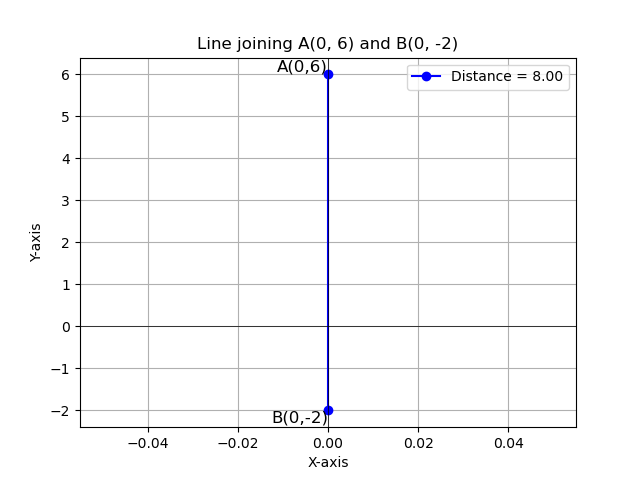
\includegraphics[width=0.7\linewidth]{figs/dist.png}
	\caption{Line joining $\vec{A}$ and $\vec{B}$}
   \end{figure}
   \end{document}

